\documentclass[4pt]{article}
\title{\LARGE {Analytic of VPT in iron-based superconductor}}
\author{\Large{Wei Cheng}}
\date{\Large{}}
\usepackage{amsmath,amsthm,amssymb,amsfonts, fancyhdr, color, comment, graphicx, environ}
\usepackage{verbatim}
\usepackage[UTF8]{ctex}%用于识别中文
\usepackage{underscore}%可以用来正确识别_
\usepackage{graphicx}%用于插入图片
\usepackage{geometry}
\usepackage{braket}
\usepackage{listing}
\geometry{a4paper,scale=0.85}
\usepackage{hyperref}%用于插入链接
\hypersetup{
	colorlinks=true,
	linkcolor=blue,
	filecolor=magenta,      
	urlcolor=blue,
}%插入链接的性质
\usepackage{pythontex}
\usepackage{import}
\usepackage{subfiles}
\usepackage{xifthen}
\usepackage{pdfpages}
\usepackage{transparent}
\usepackage{framed}
\usepackage{tcolorbox}
\usepackage[dvipsnames,svgnames]{xcolor}
\usepackage{abstract}
\usepackage{pgfplots,tikz}
\tcbuselibrary{skins,breakable,xparse}
\usepackage{shadowtext}
\usepackage{titlesec}
\usepackage{titletoc}
\usepackage{setspace}
\usepackage{float}
\usepackage{enumitem}  
\usepackage[normalem]{ulem}
\usepackage[charter]{mathdesign}
\usepackage{shadowtext}
\usepackage{setspace}
\usepackage{tabularcalc}
\usepackage{booktabs}
\usepackage[citecolor=red]{hyperref}%用于插入链接
\hypersetup{
	colorlinks=true,
	linkcolor=blue,
	filecolor=red,      
	urlcolor=blue,
	citecolor=red
}%插入链接的性质
\usepackage{ragged2e}




\renewcommand{\abstractname}{\Large Abstract}
\renewcommand\refname{\LARGE Reference}




\definecolor{mygreen}{rgb}{0.8,1,0.73}
\definecolor{linegreencolor}{rgb}{0,0.4,0}
\definecolor{myblue}{rgb}{0.22,0.73,0.91}
\definecolor{LightBlue1}{rgb}{0.22,0.73,0.91}
\definecolor{myteal}{cmyk}{0.5,0,0.15,0}
\definecolor{myred}{RGB}{255,182,185}
\definecolor{myredline}{RGB}{228,44,100}

\titleformat*{\section}{\Large\bfseries\filcenter}
\titleformat*{\subsection}{\Large\bfseries}
\titleformat*{\subsubsection}{\Large\bfseries}
\titleformat*{\paragraph}{\large\bfseries}
\titleformat*{\subparagraph}{\large\bfseries}

\renewcommand*\contentsname{\hfill \LARGE{Content} \hfill}

\newcommand{\upcite}[1]{\textsuperscript{\textsuperscript{\cite{#1}}}}
\begin{document}
		\maketitle
		\large
		From the analysis,we want to understand change the sign of the $A_z$ will cause the topological phase transition from two to one.For simpilify we choose vortex along the z direction.
		\par 
		In the basics $\ket{p_z,\uparrow},\ket{p_z,\downarrow},\ket{d_{xz+iyz},\downarrow},\ket{d_{xz-iyz},\uparrow},\ket{d_{xz+iyz},\uparrow},\ket{d_{xz-iyz,\downarrow}}$,we consider the$k_z=0$
	\begin{align}
		H=
		\begin{pmatrix}
			M(k) &0&0 &-iAk_{-} &-iAk_{+}&0\\
			0&M(k)&-iAk_{+}&0&0&-iAk_{-}\\
			0&iAk_{-}&-M(k)&0&0&0\\
			iAk_{+}&0&0&-M(k)&0&0\\
			iAk_{-}&0&0&0&-M(k)+\delta&0\\
			0&iAk_{+}&0&0&0&-M(k)+\delta
		\end{pmatrix}
	\end{align}
	$M(k)=M_0+M_1(k_x^2+k_y^2),k_{+}=k_x+ik_y,k_{-}=k_x-ik_y$
	we can do a transformation to diagonalization
	the Hamiliton
	\begin{align}
		U=
		\begin{pmatrix}
			1&0&0&0&0&0\\
			0&0&0&1&0&0\\
			0&0&0&0&1&0\\
			0&1&0&0&0&0\\
			0&0&1&0&0&0\\
			0&0&0&0&0&1\\
		\end{pmatrix}
	\end{align}
	Finally we can get the block from is
	\begin{align}
		H_k=
		\begin{pmatrix}
			M(k)&-iAk_{-}&-iAk_{+}&&&\\
			iAk_{+}&-M(k)&0&&&\\
			iAk_{-}&0&-M(k)+\delta&&&\\
			&&&M(k)&-iAk_{+}&-iAk_{-}\\
			&&&iAk_{-}&-M(k)&0\\
			&&&iAk_{+}&0&-M(k)
		\end{pmatrix}
	\end{align}
we can get the electron in the basics $\{\ket{p_z,\uparrow}_e,\ket{d_{xz-iyz},\uparrow}_e,\ket{d_{xz+iyz},\uparrow}_e\}$,the Hamiliton is 
\begin{align}
	H_{e\uparrow}(k)=
	\begin{pmatrix}
		M(k)&-iAk_{-}&-iAk_{+}\\
		iAk_{+}&-M(k)&0\\
		iAk_{-}&0&-M(k)\\
	\end{pmatrix}
\end{align}
	In the $\{\ket{p_z,\downarrow}_e,\ket{d_{xz+iyz},\downarrow}_e,\ket{d_{xz-iyz},\downarrow}_e\}$ the Hamiliton is 
\begin{align}
	H_{e\downarrow}(k)=
		\begin{pmatrix}
		M(k)&-iAk_{+}&-iAk_{-}\\
		iAk_{-}&-M(k)&0\\
		iAk_{+}&0&-M(k)\\
	\end{pmatrix}
\end{align}
The we can do the particle-hole transformation to get the Hamiliton in the hole space $\{\ket{p_z,\downarrow}_h,\ket{d_{xz+iyz},\downarrow}_h,\ket{d_{xz-iyz},\downarrow}_h\}$
\begin{align}
	H_{h\downarrow}(k)=-H_{e\downarrow}^{*}(-k)=
	-
	\begin{pmatrix}
			M(k)&-iAk_{+}&-iAk_{-}\\
			iAk_{-}&-M(k)&0\\
			iAk_{+}&0&-M(k)\\
	\end{pmatrix}
=-H_{e\uparrow}(k)
\end{align}
	Then we can solve the eigenvalue and eigenwave function for $H_{e\uparrow}(k)$,for simpilify,we can write it in the polar coordinate,we can get the $H_{e\uparrow}(k)$ is
	\begin{align}
		H_{e\uparrow}(k)=
		\begin{pmatrix}
			M(k)&-iAke^{-i\theta}&-iAke^{i\theta}\\
			iAke^{i\theta}&-M(k)&0\\
			iAke^{-i\theta}&0&-M(k)
		\end{pmatrix}
	\end{align}
	we can get the three eigenvalue
	\begin{align}
		E_{\pm}=\pm\sqrt{M(k)^2+2A^2k^2} \qquad E_0=-M(k)
	\end{align}
	We can see that the eigenvalue is only relate to the length of k,independent of theta,so we can definit a angular momentum
	\begin{align}
		J_z=-i\partial_{\theta}+J_{basis}=-i\partial_{\theta}+
		\begin{pmatrix}
			\frac{1}{2}&&\\
			&-\frac{1}{2}&\\
			&&\frac{3}{2}
		\end{pmatrix}
	\end{align}
For the orbit angular momentum,we can write it in p appearance
\begin{align}
	L_z=(\vec{r}\times\vec{p})_z&=xp_y-yp_x\\
	&=ip_y\partial_{p_x}-ip_x\partial_{p_y}
\end{align}
	In the coordinate of the p 
	\begin{align}
		\partial_{p_x}=cos(\theta)\partial_{p}-\frac{1}{p}sin(\theta)\partial_{\theta}\\
		\partial_{p_y}=sin(\theta)\partial_{p}+\frac{1}{p}cos(\theta)\partial_{\theta}
	\end{align}
Then we can get 
\begin{align}
	L_z&=ip_y\partial_{p_x}-ip_x\partial_{p_y}\\
	&=ipsin(\theta)[cos(\theta)\partial_{p}-\frac{1}{p}sin(\theta)\partial_{\theta}]-ipcos(\theta)	[sin(\theta)\partial_{p}+\frac{1}{p}cos(\theta)\partial_{\theta}]\\
	&=-i\partial_{\theta}
\end{align}
Due to $[H_{e\uparrow}(k),J_z]=0$,we can get the common eigen states of the $H_{e\uparrow}(k)$ and $J_z$
\begin{align}
	\psi(k,\theta)^j=
	\begin{pmatrix}
			e^{i(j-\frac{1}{2})\theta}u_1(k)\\
			e^{i(j+\frac{1}{2})\theta}u_2(k)\\
			e^{i(j-\frac{3}{1})\theta}u_3(k)
	\end{pmatrix}
\end{align}	
	Then we can definite a unitary transformation
	\begin{align}
		U=
		\begin{pmatrix}
			e^{i(j-\frac{1}{2})\theta}&&\\
			&e^{i(j+\frac{1}{2})\theta}&\\
			&&e^{i(j-\frac{3}{2})\theta}
		\end{pmatrix}
	\end{align}
The we can get 
\begin{align}
	U^{\dagger}H_{e\uparrow}(k)U=
	\begin{pmatrix}
		M(k)&-iAk&-iAk\\
		iAk&-M(k)&0\\
		iAk&0&-M(k)
	\end{pmatrix}
\end{align}
	we can solve the eigen states
	\begin{align}
		\ket{\psi_0}=\frac{1}{\sqrt{2}}
		\begin{pmatrix}
			0\\
			-1\\
			1
		\end{pmatrix}
	\qquad
		\ket{\psi_{\pm}}=\frac{1}{a_{\pm}}
		\begin{pmatrix}
			-i(M(k)\pm E)\\
			Ak\\
			Ak
		\end{pmatrix}
	\end{align}
The$E=\sqrt{M(k)^2+2A^2k^2},a_{\pm}$is normalization constant,then we can get the eigen states of angular momentum j is
\begin{align}
	\ket{\psi_0^j}_e=\frac{1}{2\sqrt{\pi}}
	\begin{pmatrix}
		0\\
		-e^{i(j+\frac{1}{2})\theta}\\
		e^{i(j-\frac{3}{2}\theta)}
	\end{pmatrix}
\qquad
	\ket{\psi_{\pm}^j}_e=\frac{1}{a_{\pm}\sqrt{2\pi}}
	\begin{pmatrix}
		-i(M(k)\pm E)e^{i(j-\frac{1}{2})\theta}\\
		Ake^{i(j+\frac{1}{2})\theta}\\
		Ake^{i(j-\frac{3}{2})\theta}
	\end{pmatrix}
\end{align}
For the hole part,because$H_{h\downarrow}(k)=-H_{e\uparrow}(k)$,use the same way to calculate,we can find it's eigen value is negative to the electronic part, it's eigen states will correspondenced to electronic part.
\begin{align}
	\ket{\psi_0^j}_h=\frac{1}{2\sqrt{\pi}}
	\begin{pmatrix}
		0\\
		-e^{i(j+\frac{1}{2})\theta}\\
		e^{i(j-\frac{3}{2}\theta)}
	\end{pmatrix}
	\qquad
	\ket{\psi_{\pm}^j}_h=\frac{1}{a_{\pm}\sqrt{2\pi}}
	\begin{pmatrix}
		-i(M(k)\pm E)e^{i(j-\frac{1}{2})\theta}\\
		Ake^{i(j+\frac{1}{2})\theta}\\
		Ake^{i(j-\frac{3}{2})\theta}
	\end{pmatrix}
\end{align}
		For simpilify,we can choose$j=\frac{1}{2}$,we can get
\begin{align}
	\ket{\psi_0}_e=\frac{1}{2\sqrt{\pi}}
	\begin{pmatrix}
		0\\
		-e^{i\theta}\\
		e^{-i\theta}
	\end{pmatrix}
	\qquad
	\ket{\psi_{\pm}}_e=\frac{1}{a_{\pm}\sqrt{2\pi}}
	\begin{pmatrix}
		-i(M(k)\pm E)\\
		Ake^{i\theta}\\
		Ake^{-i\theta}
	\end{pmatrix}
\end{align}
\begin{align}
	\ket{\psi_0}_h=\frac{1}{2\sqrt{\pi}}
	\begin{pmatrix}
		0\\
		-e^{i\theta}\\
		e^{-i\theta)}
	\end{pmatrix}
	\qquad
	\ket{\psi_{\pm}}_h=\frac{1}{a_{\pm}\sqrt{2\pi}}
	\begin{pmatrix}
		-i(M(k)\pm E)\\
		Ake^{i\theta}\\
		Ake^{-i\theta}
	\end{pmatrix}
\end{align}	
	We can choose the parameter $M_0=-1,M_1=1,A=0.5$,we can plot the band structure along the $k_x$ direction(because we consider the system has circle rotation symmetry,so along the any direction of the $k_x-k_y$plane,we will get the same band structure.)
	\begin{figure}[ht]
		\centering
		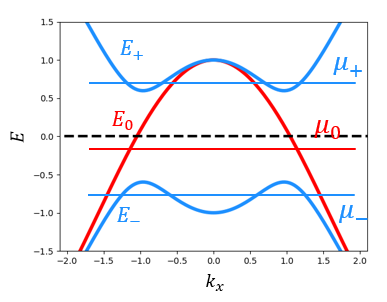
\includegraphics[scale=1]{figure/1}
	\end{figure}
When the Fermi surface near the $\mu_0$,Only one band near Fermi surace, so we can project $H_{BdG}$ to this band,it means that we can write $H_{BdG}$ on the $\{\ket{\psi_0}_e,\ket{\psi_0}_h\}$ basics.
	\begin{align}
		H_{BdG}^{00}=
		\begin{pmatrix}
		E-\mu & i\Delta_ee^{-i\theta}(\partial_k-\frac{i\partial_{\theta}+A_{\theta}^{00}}{k})\\
		i\Delta_ee^{i\theta}(\partial_k+\frac{i\partial_{\theta}+A_{\theta}^{00}}{k})& \mu-E
	\end{pmatrix}
	\end{align}
The vortex will not break the rotation symmetry on the $x-y$ plane,so we can define the angular momentum
	\begin{align}
		J_z=L_z+J_{basis}+J_{vortex}=-i\partial_{\theta}+\frac{1}{2}+\frac{1}{2}\tau_z
	\end{align}
	The eigne wave function is
	\begin{align}
			\psi(k,\theta)=\frac{1}{\sqrt{k}}
			\begin{pmatrix}
				e^{i(j-1)\theta }u_1(k)\\
				-ie^{ij\theta}u_2(k)
			\end{pmatrix}
	\end{align}
	so we can do the unitary transformation
	\begin{align}
		U=\begin{pmatrix}
			e^{i(j-1)\theta}&\\
			&-ie^{ij\theta}
		\end{pmatrix}
	\end{align}
	Then we can get
	\begin{align}
		(H_{BdG}^{00})^j=U^{\dagger}H_{BdG}^{00}U
		&=\begin{pmatrix}
			E-\mu &\Delta_e(\frac{j-\frac{1}{2}-A_{\theta}^{00}}{k}+\partial_k)\\
			\Delta_e(\frac{j-\frac{1}{2}-A_{\theta}^{00}}{k}-\partial_k) &\mu-E
		\end{pmatrix}\\
	&=(E-\mu)\sigma_z+i\Delta_e\partial_k+\frac{\Delta_e}{k}(j-\frac{1}{2}-A_{\theta}^{00})
	\end{align}
The resulting Hamiltonian is equivalent to the
Jackiw-Rebbi model,so we can get 
	\begin{align}
		E_j=\frac{\Delta_e}{k}(j-\frac{1}{2}-A_{\theta}^{00})
	\end{align}
we can calculate $A_{\theta}^{00}=i_e\bra{\psi_0}\partial_{\theta}\ket{\psi_0}_h=-1$,so $E_j$ is impossible to be zero,so we can conclude that it's will not have vortex transition point near the $\mu_0$
\par 
When the Fermi surface near the $\mu_{-}$,there will have two band $E_0,E_{-}$ near the Fermi surface ,we can project $H_{BdG}$ to this two band.
For simipilify calculte,we can do a transformation from $(k,\theta) to (E,\theta)$,Then we can write $H_{BdG}$ in the basics $\{\ket{\psi_0(E,\theta)}_e,\ket{\psi_{-}(E,\theta)}_e,\ket{\psi_0(E,\theta)}_h,\ket{\psi_{-}}(E,\theta)_h\}$
\begin{align}
	\begin{pmatrix}
		E-\mu &&\Delta_{11} &\Delta_{12}\\
		&E-\mu&\Delta_{21} &\Delta_{22}\\
		\Delta_{11}^{\dagger}&\Delta_{12}^{\dagger}&\mu-E&\\
		\Delta_{21}^{\dagger}&\Delta_{22}^{\dagger}&&\mu-E
	\end{pmatrix}
\end{align}
The elements is
\begin{align}
	\Delta_{11}&=i\Delta_ee^{-i\theta}(\frac{dE}{dk_{-}}\partial_{E}-\frac{i\partial_{\theta}+A_{\theta}^{00}}{k_{-}(E)})\\
	&=i\Delta_ee^{-i\theta}(\hbar v_{k_{-}}\partial_{E}-\frac{i\partial_{\theta}+A_{\theta}^{00}}{k_{-}(E)})
\end{align}
\begin{align}
	\Delta_{12}&=_e\bra{\psi_0(k_0,\theta)}\Delta_0tanh(\frac{r}{\xi})e^{-i\theta}\ket{\psi_{-}(k_{-},\theta)}_h\\
	&=_e\bra{\psi_0(k_0,\theta)}\Delta_ere^{-i\theta}\frac{tanh(\frac{r}{\xi})}{\frac{r}{\xi}}\ket{\psi_{-}(k_{-},\theta)}_h\\
	&=-\frac{\Delta_e}{k_{-}}A_{\theta}^{12}_e\bra{\psi_0(k_0,\theta)}\frac{tanh(\frac{r}{\xi})}{\frac{r}{\xi}}\ket{\psi_{-}(k_{-},\theta)}_h
\end{align}
The right integral can be calculate by numeral calculations,we can get 
	\begin{figure}[H]
	\centering
	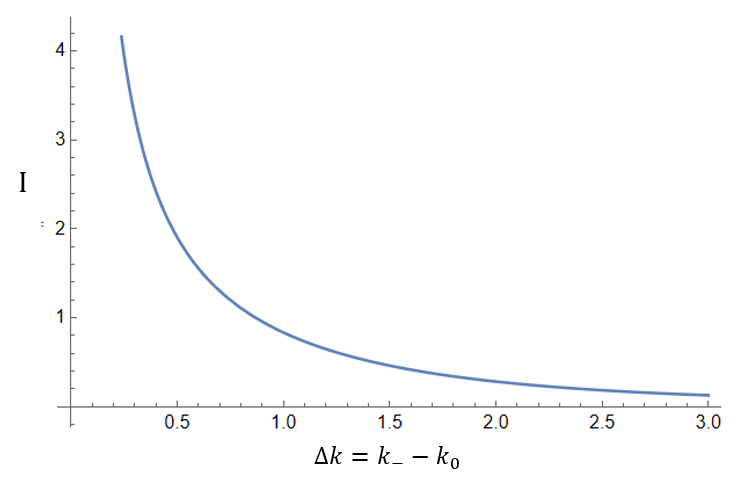
\includegraphics[scale=0.7]{figure/2}
\end{figure}
The horizontal axis representation the difference of the $k_0$ and $k_{-}$,we can see that the more difference,the little integral.So we can only consider the interaction of the nearst k.For simpilify we can treat this integral as a correction on $k_{-}$,we can change $k_{-}$ to $k_{m}=\frac{k_0+k_{-}}{2}$,Then we can get
\begin{align}
	\Delta_{12}=-\frac{\Delta_e}{k_m}A_{\theta}^{12}
\end{align}
At the same time
\begin{align}
	\Delta_{22}=i\Delta_ee^{-i\theta}(\hbar v_{k_{-}}\partial_E-iA_E^{22}-\frac{i\partial_{\theta+A_{\theta}^{22}}}{k})
\end{align}
we can do the gauge transfomation $\ket{\psi_{-}(E,\theta)}\rightarrow e^{i\int^EA_{E^{'}}^{22}}dE^{'}$ to eliminate $A_{E}^{22}$,The we can get the form of the project $H_{BdG}$,For easy to calculate,we can write the $H_{BdG}$ in the basics $\{\ket{\psi_0(E,\theta)}_e,\ket{\psi_0(E,\theta)}_h,\ket{\psi_{-}(E,\theta)}_e,\ket{\psi_{-}}(E,\theta)_h\}$
\begin{align}
	\begin{pmatrix}
		E-\mu &i\Delta_ee^{-i\theta}(\hbar v_{k_{-}}\partial_E-\frac{i\partial_{\theta}+A_{\theta}^{00}}{k_{-}(E)})&0&-\frac{\Delta_e}{k_m}e^{-i\theta}A_{\theta}^{0-}\\
		i\Delta_ee^{i\theta}(\hbar v_{k_{-}}\partial_{E}+\frac{i\partial_{\theta}+A_{\theta}^{00}}{k})&\mu-E&-\frac{\Delta_e}{k_m}e^{i\theta}A_{\theta}^{-0}&0\\
		0&-\frac{\Delta_e}{k_m}e^{-i\theta}A_{\theta}^{0-}&E-\mu&i\Delta_ee^{-i\theta}(\hbar v_{k_{-}}\partial_E-\frac{i\partial_{\theta}+A_{\theta}^{--}}{k_{-}(E)})\\
		-\frac{\Delta_e}{k_m}e^{i\theta}A_{\theta}^{-0}&0&	i\Delta_ee^{i\theta}(\hbar v_{k_{-}}\partial_{E}+\frac{i\partial_{\theta}+A_{\theta}^{--}}{k})&E-\mu
	\end{pmatrix}
\end{align}
The $H_{BdG}$ has the rotation symmetry,so we can definite the angular momentum 
\begin{align}
	J_z=-i\partial_{\theta}+\frac{1}{2}+\frac{1}{2}\tau_z
\end{align}
The egie wave function is
\begin{align}
	\psi(E,\theta)=\frac{1}{\sqrt{k_{-}(E)}}
	\begin{pmatrix}
					e^{i(j-1)\theta}u_1(k)\\
					-ie^{ij\theta}u_2(k)\\
					e^{i(j-1)\theta}u_3(k)\\
					-ie^{ij\theta}u_4(k)
	\end{pmatrix}
\end{align}
So we can do a unitary transformation
\begin{align}
	U=\frac{1}{\sqrt{k_{-}(E)}}
	\begin{pmatrix}
		e^{i(j-1)\theta}&&&\\
		&-ie^{ij\theta}&&\\
		&&e^{i(j-1)\theta}&\\
		&&&-ie^{ij\theta}
	\end{pmatrix}
\end{align}
Then we can get 
\begin{equation}
	\begin{pmatrix}
		E-\mu &\Delta_e(\hbar v_{k_{-}}\partial_E+\frac{j-\frac{1}{2}-A_{\theta}^{00}}{k})&0&-\Delta_e\frac{A_{\theta}^{0-}}{k}\\
-		\Delta_e(\frac{j-\frac{1}{2}-A_{\theta}^{00}}{k}-\hbar v_{k_{-}\partial_E)&\mu-E&-\Delta_e\frac{A_{\theta}^{0-}}{k}&0\\
			0&-\Delta_e\frac{A_{\theta}^{-0}}{k}&E-\mu&\Delta_e(\hbar v_{k_{-}}\partial_E+\frac{j-\frac{1}{2}-A_{\theta}^{--}}{k})\\
				-\Delta_e\frac{A_{\theta}^{-0}}{k}&0&\Delta_e(\frac{j-\frac{1}{2}-A_{\theta}^{--}}{k}-\hbar v_{k_{-}}\partial_E)&\mu-E
		\end{pmatrix}\\
\end{equation}
\begin{align}
	&=(E-\mu)s_0\tau_z+i\Delta_e\hbar v_{k_{-}}\partial_Es_0\tau_y+\frac{\Delta_e}{k_{-}(E)}(j-\frac{1}{2})s_0\tau_x-
	\begin{pmatrix}
		0&\frac{\Delta_e}{k_{-}(E)}A_{\theta}^{00}&0&\frac{\Delta_e}{k_m}A_{\theta}^{0-}\\
		\frac{\Delta_e}{k_{-}(E)}A_{\theta}^{00}&0&\frac{\Delta_e}{k_m}A_{\theta}^{0-}&0\\
		0&\frac{\Delta_e}{k_m}A_{\theta}^{-0}&0&\frac{\Delta_e}{k_{-}(E)}A_{\theta}^{--}\\
		\frac{\Delta_e}{k_m}A_{\theta}^{-0}&0&\frac{\Delta_e}{k_{-}(E)}A_{\theta}^{--}&0
	\end{pmatrix}\\
&=(E-\mu)s_0\tau_z+i\Delta_e\hbar v_{k_{-}}\partial_{E}s_0\tau_y+\frac{\Delta_e}{k_{-}(E)}[(j-\frac{1}{2})s_0-\begin{pmatrix}
	A_{\theta}^{00} & \frac{k_{-}(E)}{k_m}A_{\theta}^{0-}\\
	\frac{k_{-}(E)}{k_m}A_{\theta}^{-0}&A_{\theta}^{--}
\end{pmatrix}]\tau_x
\end{align}
The resulting Hamiltonian is equivalent to the
$4*4$Jackiw-Rebbi model,we can solve the zero solution of the first two items
\begin{align}
	\psi_0^{1}(E)=\frac{1}{2}e^{\int^{E}\frac{\mu-E^{'}}{\Delta_e\hbar v_{k_{-}}}dE^{'}}
	\begin{pmatrix}
		1\\
		1\\
		1\\
		1
	\end{pmatrix}
\end{align}
\begin{align}
	\psi_0^{2}(E)=\frac{1}{2}e^{\int^{E}\frac{\mu-E^{'}}{\Delta_e\hbar v_{k_{-}}}dE^{'}}
	\begin{pmatrix}
		1\\
		1\\
		-1\\
		-1
	\end{pmatrix}
\end{align}
we can calculate that 
\begin{align}
	A_{\theta}^{00}=0 \qquad A_{\theta}^{--}=0 \qquad A_{\theta}^{0-}=\frac{\sqrt{2}Ak_{-}(E)}{a_{-}}
\end{align}
The energy can be determined by 
\begin{align}
	H_j=\frac{\Delta_e}{k_{-}(E)}(j-\frac{1}{2})s_0\tau_x-\frac{\Delta_e}{k_m}A_{\theta}^{0-}s_x\tau_x
\end{align}
Then we can get the eigen value
\begin{align}
E_j=\frac{\Delta_e}{k_{-}(E)}(j-\frac{1}{2}\pm \frac{k_{-}(E)}{k_m}A_{\theta}^{0-})
\end{align}
It's eigen value is $(1,1,1,1)^T$ and $(1,1,-1,-1)^T$
corresponed to the zero solution of the Jackiw-Rebbi model.If we want to get the zero solution,we need to require $\frac{k_{-}(E)}{k_m}A_{\theta}^{0-}$ be a half integer,we can easily to analysis that $\frac{k_{-}(E)}{k_m}A_{\theta}^{0-}$ more than zero and less than 1,so the only possible is to be $\frac{1}{2}$,Then we can get the zero solution's angular must be 0 or 1,Then we can get the zero solution 
\begin{align}
	\psi_0^{j=0}(E,\theta)=\frac{1}{2\sqrt{k_{-}(E)}}e^{\int^E\frac{\mu-E^{'}}{\Delta_e\hbar v_{k_{-}}}dE^{'}}
	\begin{pmatrix}
		e^{-i\theta}\\
		-i\\
		e^{-i\theta}\\
		-i
	\end{pmatrix}
\end{align}
\begin{align}
	\psi_0^{j=1}(E,\theta)=\frac{1}{2\sqrt{k_{-}(E)}}e^{\int^E\frac{\mu-E^{'}}{\Delta_e\hbar v_{k_{-}}}dE^{'}}
	\begin{pmatrix}
		1\\
		-ie^{i\theta}\\
		-1\\
		ie^{i\theta}
	\end{pmatrix}
\end{align}
At the same time,we can calculate the vortex phase transition energy,we can get 
\begin{align}
	\frac{k_{-}(E)}{k_m}A_{\theta}^{0-}=\frac{k_{-}(E)}{\frac{k_{0}(E)+k_{-}(E)}{2}}\frac{\sqrt{2}Ak_{-}(E)}{a_{-}}=\frac{1}{2}
\end{align}
we can bring the parameter into equation,it's the $M0=-1,M1=1,A=0.5$,for simpilify,we can estimate $\frac{k_{-}(E)}{\frac{k_{0}(E)+k_{-}(E)}{2}}$ to be a constant 0.81,Finally we can get it's vortex phase transition at E=-0.79,At the same time,we can get When the Fermi surface near the $\mu_{+}$,it's vortex phase transition point at E=0.66.
\par 
So from the analysis,we can get there will have four vortex phase transition point,two of them have the 0 angular momentum,other have +1 angular momentum, and the vortex phase transition energy at $E_{+}=0.66$,$E_{-}=-0.79$,there are all correspondence to numerical calculation.

\par 

\begin{figure}[H]
	\centering
	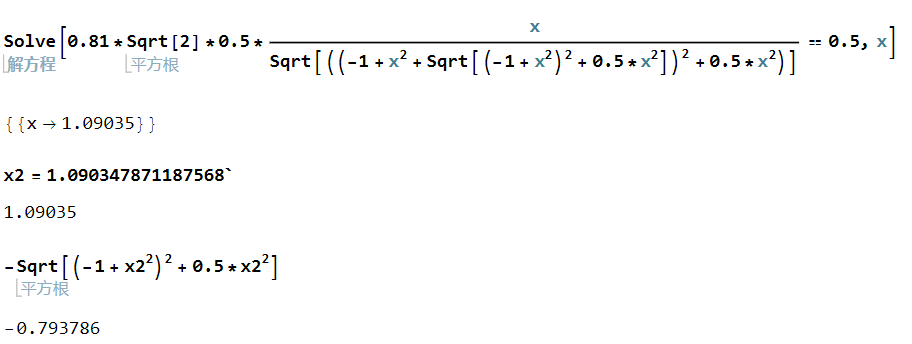
\includegraphics[scale=0.6]{figure/3}
\end{figure}
\begin{figure}[H]
	\centering
	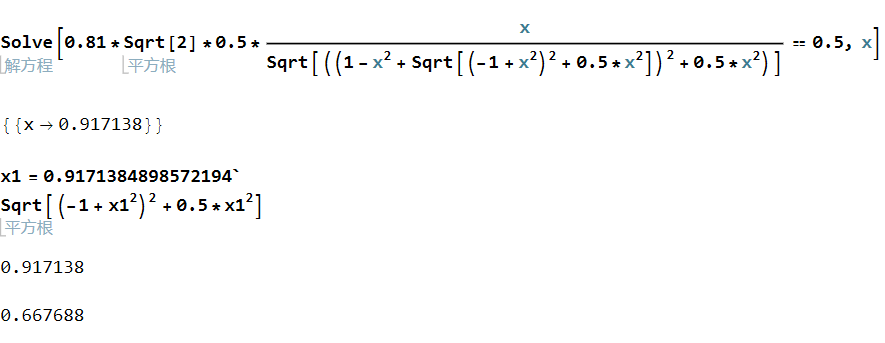
\includegraphics[scale=0.6]{figure/4}
\end{figure}

\begin{figure}[H]
	\centering
	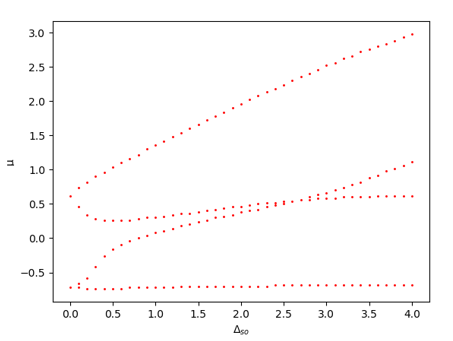
\includegraphics[scale=0.6]{figure/5}
\end{figure}

When change the sign of parameter of the $k_y$,the Hamiliton change to

When we change the sign of ky's parameter in Dirac semimetal,the electron Hamiliton become

\begin{align}
	H_{e\uparrow}(k)=
	\begin{pmatrix}
		M(k) & -iAke^{-i\theta}&-iAke^{-i\theta}\\
		iAke^{i\theta}&-M(k)&0\\
		iAke^{i\theta}&0&-M(k)
	\end{pmatrix}
\end{align}

We can definite the angular momentum

Now the angular momentum become

\begin{align}
	J_z=-i\partial_{\theta}+\begin{pmatrix}
		\frac{1}{2}&&\\
		&-\frac{1}{2}&\\
		&&-\frac{1}{2}
	\end{pmatrix}
\end{align}

We can use the same way to get the eige states of the $H_{e\uparrow}(k)$

Use the same way,we can solve the eigen states of the $H_{e\uparrow}(k)$

\begin{align}
	\ket{\psi_0^j}_e=\frac{1}{2\sqrt{\pi}}
	\begin{pmatrix}
		0\\
		-e^{i(j+\frac{1}{2})\theta}\\
		e^{i(j+\frac{1}{2}\theta)}
	\end{pmatrix}
	\qquad
	\ket{\psi_{\pm}^j}_e=\frac{1}{a_{\pm}\sqrt{2\pi}}
	\begin{pmatrix}
		-i(M(k)\pm E)e^{i(j-\frac{1}{2})\theta}\\
		Ake^{i(j+\frac{1}{2})\theta}\\
		Ake^{i(j+\frac{3}{2})\theta}
	\end{pmatrix}
\end{align}
For the hole part
\begin{align}
	\ket{\psi_0^j}_h=\frac{1}{2\sqrt{\pi}}
	\begin{pmatrix}
		0\\
		-e^{i(j+\frac{1}{2})\theta}\\
		e^{i(j+\frac{1}{2}\theta)}
	\end{pmatrix}
	\qquad
	\ket{\psi_{\pm}^j}_h=\frac{1}{a_{\pm}\sqrt{2\pi}}
	\begin{pmatrix}
		-i(M(k)\pm E)e^{i(j-\frac{1}{2})\theta}\\
		Ake^{i(j+\frac{1}{2})\theta}\\
		Ake^{i(j+\frac{1}{2})\theta}
	\end{pmatrix}
\end{align}
For simpilify to calculate,we can choose $j=-\frac{1}{2}$
\begin{align}
	\ket{\psi_0}_e=\frac{1}{2\sqrt{\pi}}
	\begin{pmatrix}
		0\\
		-1\\
		1
	\end{pmatrix}
	\qquad
	\ket{\psi_{\pm}}_e=\frac{1}{a_{\pm}\sqrt{2\pi}}
	\begin{pmatrix}
		-i(M(k)\pm E)e^{-i\theta}\\
		Ak\\
		Ak
	\end{pmatrix}
\end{align}
\begin{align}
	\ket{\psi_0}_h=\frac{1}{2\sqrt{\pi}}
	\begin{pmatrix}
		0\\
		-1\\
		1
	\end{pmatrix}
	\qquad
	\ket{\psi_{\pm}}_h=\frac{1}{a_{\pm}\sqrt{2\pi}}
	\begin{pmatrix}
		-i(M(k)\pm E)e^{-i\theta}\\
		Ak\\
		Ak
	\end{pmatrix}
\end{align}	
We can notice that $\ket{\psi_0}_e$ is independent of the $k$ and $\theta$,so the it's connection of the other band must zero,so we just to consider one band model.For example, When Fermi energy near the $\mu_{-}$,the eigne energy is   
\begin{align}
	E_j=\frac{\Delta_e}{k}(j-\frac{1}{2}-A_{\theta}^{--})
\end{align}
If we want to get the zero solution,we need the $A_{\theta}^{--}$ is the half of integer,we can get 
\begin{align}
	A_{\theta}^{--}=\frac{(-M(k)+E)^2}{(-M(k)+E)^2+2A^2k^2}
\end{align}
From easily analysis,if the  $A_{\theta}^{--}$ is the half of integer,it must be $\frac{1}{2}$.we can get when $M(k)=0$,the  $A_{\theta}^{--}=\frac{1}{2}$.We can take the parameter into this equation,we can get the vortex phase traansition energy is $\pm 0.707$,and the angular momentum is $j=1$,so the $C_{2z}$ is -1.This result is  corresponding the numerical result too.
\begin{figure}[H]
	\centering
	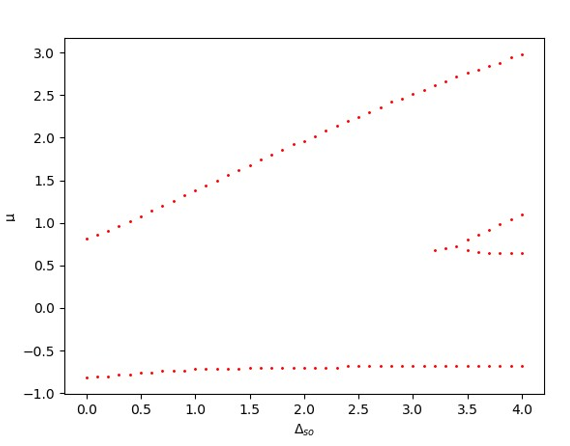
\includegraphics[scale=0.6]{figure/6}
\end{figure}

When change the parameter of $k_y$ to zero,it says that the Hamiliton change to 
\begin{align}
		H_{e\uparrow}(k)=
		\begin{pmatrix}
					M(k) & -iAk_{-} &-iAk_{x}\\
					iAk_{+} &-M(k) &0\\
					iAk_{x}&0&-M(k)
		\end{pmatrix}
\end{align}
we can solve it's eigenvalue and eigenstates
\begin{align}
	E_{0}=-M(k) \qquad E_{\pm}=\pm \sqrt{M(k)^2+2A^2k_x^2+A^2k_y^2}
\end{align}

\begin{align}
	\psi_0=\frac{1}{\sqrt{3\pi}}
	\begin{pmatrix}
		0\\
		-cos\theta\\
		e^{-i\theta}
	\end{pmatrix}
\qquad 
	\psi_{\pm}=\frac{1}{a_{\pm}}
\begin{pmatrix}
		-i(M(k)\pm E)\\
		Ake^{i\theta}\\
		Akcos\theta
\end{pmatrix}
\end{align}
The normalization coefficient is
\begin{align}
	a_{\pm}&=\int_0^{2\pi}A^2k^2cos\theta^2+A^2k^2+(M(k)\pm E)^2 d\theta \\
	&=3\pi A^2k^2+2\pi M(k)+\int_0^{2\pi}\sqrt{M(k)^2+A^2k^2+A^2k^2cos\theta^2}d\theta\\
	&=3\pi A^2k^2+2\pi M(k)+\alpha (k)
\end{align}
At this time,we can find the $E_{0}$ is isotropic,but the $E_{\pm}$ is anisotropy.For simpilify to estimate,we can just think $E_{\pm}$ is isotropic.The we can use the same way of the calculation, we assume that the fermi surface is near the $\mu_{0}$
we can get the 
\begin{align}
	A_{\theta}^{00}=i\bra{\psi_0}\partial_{\theta}\ket{\psi_0}=\frac{2}{3}
\end{align}
so it can't be a half of integer , so the middle band can't have a vortex phase transition point.
\par 
we next assume that the fermi surface is near the $\mu_{-}$,we can calculate that 
 

\end{document}